\section*{Oppgave 2 - Interpolated Precision}
\subsection*{Deloppgave a}
Interpolated precision er noe som brukes når man ønsker å lage en mer meningsfylt Recall-Precision graf. Den fungerer ved at man setter en presisjon for et intervall med recall istede for å ha en presisjon for alle recall verdier, noe som gjør at man får en svært hakkete graf. Dette fungerer godt fordi brukeren sannsynligvis vil sjekke ut flere relevante dokumenter og da er det grei å kjøre den høyeste gitte presisjons-verdien for et recall-intervall.

\pagebreak
\subsection*{Deloppgave b}

Gitt de følgende dokumententene d = \{2, 6, 72, 10, 84, 15, 103, 66, 37, 45, 12, 201, 33, 94, 22\}
og de relevante dokumentene r = \{2, 72, 103, 201, 22, 45, 33\}.
Vi var usikre på hva som mentes med de ti første dokumentene så vi har besvart oppgaven på grunnlag av alle dokumentene.
\begin{center}
    \begin{tabular}{| l | l | l | l |}
    \hline
    d & Releant & Recall & Precision \\ \hline
    2 & REL & $\frac{1}{7}$=0.14& $\frac{1}{1}$=1.0 \\ \hline
    6 &  &  & \\ \hline
    72 & REL & $\frac{2}{7}$=0.28 & $\frac{2}{3}$=0.66 \\ \hline
    10 &  &  & \\ \hline
    84 &  &  & \\ \hline
    15 &  &  & \\ \hline
    103 & REL & $\frac{3}{7}$=0.43 & $\frac{3}{7}$=0.43 \\ \hline
    66 &  &  & \\ \hline
    37 &  &  & \\ \hline
    45 & REL & $\frac{4}{7}$=0.57 & $\frac{4}{10}$=0.40 \\ \hline
    12 &  &  & \\ \hline
    201 & REL & $\frac{5}{7}$=0.71 & $\frac{5}{12}$=0.42 \\ \hline
    33 & REL & $\frac{6}{7}$=0.86 & $\frac{6}{13}$=0.46 \\ \hline
    94 &  &  & \\ \hline
    22 & REL & $\frac{7}{7}$=1.0 & $\frac{7}{15}$=0.47 \\ \hline
    \end{tabular}
\end{center}


\begin{figure}[ht!]
\centering
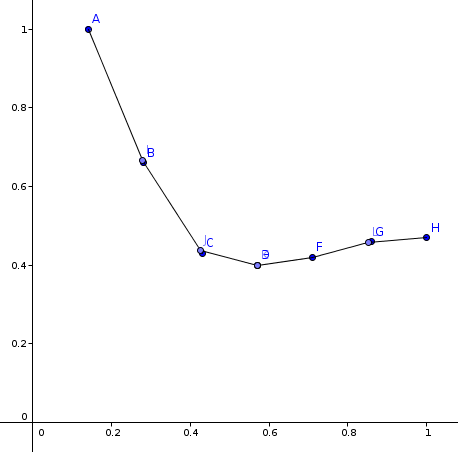
\includegraphics[scale=0.4]{interpolak.png}
\caption{Graf som representerer dataene fra oppgaven. Y-aksen representerer Precision og X-aksen representerer Recall}
\end{figure}

\pagebreak
\section*{Oppgave 3 - Relevance Feedback}
\subsection*{Deloppgave a}
Meningen med Relevance Feedback er å bruke data fra en tidligere spørring for å gi bedre presisjon av relevans på den neste spørringen. Det er vanlig å tilegne seg informasjon om den forrige spørringen var relevant for brukeren og bruke denne informsjonen. 
\subsubsection*{Query Expansion}
Query Expansion er en operasjon som gjerne brukes for å få flere relevante resultater på en gitt spørring. Det fungerer ved at logikken som tar imot spørringen kjører spørringen på flere forskjellige måter med forskjellige variasjoner av spørringen som ble motatt. Dette er svært vanlig å gjøre i søkemotorer. Endringene som er vanlig å gjøre på spørringen er for eksempel å endre ord i strengen til synonymer med samme betydning slik at man får et bredere spekter med resultater. Andre endringer kan være og rette skrivefeil og prøve forskjellige bøyninger av ordet.
\subsubsection*{Term Reweighting}
Term Reweighting går ut på å modifisere en spørring basert på resultatene den forrige spørringen fikk. Man justerer ikke selve stringen i spørringen, men man tar heller og veier alle termene i spørringen på nytt basert på forekomster av termene i resultatene på søket.
\subsubsection*{Hva er forskjellen?}
Forskjellen på term reweighting og query expansion er at term reweighting ikke endrer termene i den orginale stringen, men kun veier dem på nytt. Query expansion baserer seg på å endre stringen så den skal få flere relevante treff.

